\chapter{Network Flow}

\section{Introduzione}

Ricordiamo la struttura dei \textbf{Bipartite Matching Problems}:
\begin{myblockquote}
  Un grafo bipartito $G = (V , E)$ è un grafo non
  orientato il cui insieme di nodi può essere partizionato come
  $V = X \cup Y$, con la proprietà che ogni arco $e \in E$ ha un
  estremo in $X$ e l'altro estremo in $Y$.
\end{myblockquote}

Ora, abbiamo già visto la nozione di \textbf{matching}: abbiamo usato il
termine per descrivere raccolte di coppie su un insieme, con la
proprietà che \textbf{nessun elemento dell'insieme appare in più di una
  coppia} (si pensi ai caratteri nel Problema del
\protect\autoref{chap:seqal}.)\\

Nel caso di un grafo, gli archi costituiscono coppie di nodi, e di
conseguenza diciamo che un \textbf{matching in un grafo $G = (V , E)$
  è un insieme di archi $M \subseteq E$ con la proprietà che ogni nodo
  appare al massimo in un arco di $M$}.\\

\textbf{Un insieme di archi $M$ è un matching perfetto se ogni nodo
  appare esattamente in un arco di $M$}.\\

I matching nei grafi bipartiti possono modellare situazioni in cui gli
oggetti vengono assegnati ad altri oggetti. Un esempio sorge quando i
nodi in $X$ rappresentano i \emph{job}, i nodi in $Y$ rappresentano
le \emph{macchine} e un arco ($x_i$, $y_j$) indica che la
\emph{macchina} $y_j$ è in grado di elaborare il \emph{job} $x_i$
(\emph{job shop scheduling problem}). Un matching perfetto è, quindi, un
modo per assegnare ogni \emph{job} a una \emph{macchina} in grado di
elaborarlo, con la proprietà che a ogni \emph{macchina} è assegnato
esattamente un \emph{job}.\\

\textbf{Uno dei problemi più antichi negli algoritmi combinatori è
  quello di determinare la dimensione del matching più grande in un grafo
  bipartito G}. (Come caso particolare, si noti che $G$ ha un matching
perfetto se e solo se $|X| = |Y|$ e ha un matching di dimensione
$|X|$.)\\

Questo problema risulta essere risolvibile da un algoritmo che
gira in tempo polinomiale, ma lo sviluppo di questo algoritmo necessita
di idee fondamentalmente diverse dalle tecniche che abbiamo visto
finora.\\

Invece di sviluppare direttamente l'algoritmo, iniziamo formulando una
classe generale di problemi, i \textbf{Network Flow Problems}, che
include il Bipartite Matching Problem come caso particolare.\\

Sviluppiamo quindi un algoritmo con tempo polinomiale per un problema
generale, il problema del \textbf{Flusso Massimo (Maximum-Flow
  Problem)}, e mostriamo come questo fornisca un algoritmo efficiente
anche per il Bipartite Matching Problem.


\section{The Maximum-Flow Problem and the Ford-Fulkerson Algorithm}

Spesso si utilizzano i grafi per modellare le
\textbf{\emph{transportation networks}}, reti i cui archi trasportano
una sorta di traffico e i cui nodi fungono da ``\emph{interruttori}''
che fanno passare il traffico tra i diversi archi.

Si consideri, ad esempio, un sistema autostradale in cui gli archi sono autostrade e i nodi sono svincoli; o una rete di computer in cui gli archi sono
collegamenti che possono trasportare pacchetti e i nodi sono switch. I
modelli di rete di questo tipo hanno diversi ingredienti:

\begin{itemize}
  \item \textbf{capacità} sugli archi, che indica quanto possono trasportare;
  \item \textbf{nodi sorgente} nel grafo, che generano traffico;
  \item \textbf{nodi sink (o destinazione)} nel grafo, che possono \emph{``assorbire''} il traffico mano a mano che arriva;
  \item il \textbf{traffico}, che viene trasmesso attraverso gli archi.
\end{itemize}

\textbf{Flow Networks}: Prenderemo in considerazione grafi di questa
forma e ci riferiamo al \textbf{traffico} come \textbf{flusso},
un'entità \textbf{astratta} che viene \textbf{generata} nei \textbf{nodi
  sorgente}, trasmessa attraverso gli archi e assorbita nei \textbf{nodi
  sink}.\\

Formalmente diremo che una Flow Network è un grafo orientato
$G = (V , E)$ con le seguenti caratteristiche:


\begin{itemize}
  \item Associata a ciascun arco $e$ c'è una \textbf{capacità}, che è un numero \textbf{non negativo} che denotiamo $c_e$ .
  \item \textbf{Esiste un solo nodo sorgente} $s \in V$.
  \item \textbf{C'è \textbf{un solo nodo sink} $t \in V$.}
\end{itemize}

I nodi diversi da $s$ e $t$ saranno chiamati \textbf{nodi interni}.\\

Faremo delle assunzioni sulle reti di flusso di cui ci occupiamo:
\begin{enumerate}
  \item \textbf{Nessun arco entra nella sorgente $s$ e nessun arco esce dal
          sink $t$};
  \item Vi sia almeno un arco per ogni nodo;
  \item Tutte le capacità sono numeri interi.
\end{enumerate}

\begin{figure}[H]
  \centering
  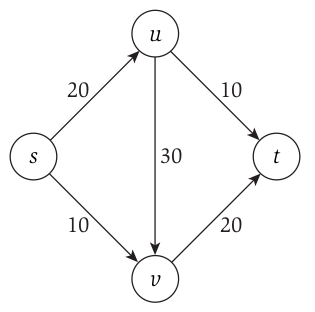
\includegraphics[width = 5cm]{capitoli/network_flow/imgs/flow1.png}
  \caption{Esempio di Flow Network}
\end{figure}

\subsection{Definizione di Flusso}

Definiamo cosa significa per la nostra rete trasportare traffico, o
flusso. Diciamo che un flusso $s-t$ è una funzione $f$ che associa
ogni arco $e$ a un numero reale non negativo, $f : E \rightarrow R^+$; il
valore $f(e)$ rappresenta la quantità di flusso trasportato dall'arco
$e$.
\\
\\
Un flusso $f$ deve soddisfare le seguenti due proprietà:
\begin{enumerate}
  \item \textbf{Capacity conditions:} Per ogni $e \in E$, abbiamo
        $0 \le f(e) \le c_e$
  \item \textbf{Conservation conditions:} Per ogni nodo $v$ diverso da $s$ e $t$, abbiamo
        $$
          \sum_{e \text{ into } v}f(e) = \sum_{e \text{ out of } v}f(e)
        $$
\end{enumerate}


Qui $\sum_{e \text{ into } v}f(e)$ somma il valore del flusso $f(e)$
su tutti gli archi che entrano nel nodo $v$, mentre
$\sum_{e \text{ out of } v}f(e)$ è la somma dei valori di flusso su
tutti gli archi che escono dal nodo $v$.
\\
\\
Quindi il flusso su un arco non può superare la capacità dell'arco
stesso. Per ogni nodo diverso dalla \textbf{source} e dal \textbf{sink},
la quantità di flusso in entrata deve essere uguale alla quantità di
flusso in uscita.

\begin{itemize}
  \item La sorgente non ha archi entranti (secondo la nostra
        assunzione), ma le è consentito avere un flusso uscente; in altre
        parole, può generare flusso.
  \item Simmetricamente, il sink può avere flusso
        in entrata, anche se non ha archi in uscita.
\end{itemize}


\textbf{Il valore di un flusso} $f$, indicato con $v(f)$, è definito
come la quantità di flusso generato alla sorgente:
$$
  v(f) = \sum_{e \text{ out of } s}f(e)
$$

Per rendere la notazione più compatta, definiamo:
$$
  f^{out}(v) = \sum_{e \text{ out of } v}f(e)
$$
$$
  f^{in}(v) = \sum_{e \text{ into } v}f(e)
$$

Possiamo estenderlo ad insiemi di vertici;

se $S \subseteq V$, definiamo $f^{out}(S) = \sum_{e \text{ out of } S}f(e)$ e
$f^{in}(S) = \sum_{e \text{ into } S}f(e)$. In questa terminologia, la
condizione di conservazione per i nodi $v \neq s, t$ diventa
$f^{in}(v) = f^{out}(v)$; e possiamo scrivere $v(f) = f^{out}(s)$.


\section{Descrizione Problema del Maximum-Flow}

Data una flow network, l'obiettivo è quello di organizzare il traffico
in modo da fare un uso il più efficiente possibile della capacità
disponibile.


\subsection{Goal}

\textbf{Data una rete di flussi, trovare un flusso di massimo valore
  possibile.}

È utile considerare come la struttura della rete di flusso pone un
\textbf{upper bound} al \textbf{valore massimo} di un flusso $s-t$.
Supponiamo quindi di dividere i nodi del grafo in due insiemi, $A$ e
$B$, in modo che $s \in A$ e $t \in B$. Allora, intuitivamente,
ogni flusso che va da $s$ a $t$ deve passare da $A$ a $B$ ad un
certo punto, e quindi consumare parte della capacità degli archi da
$A$ a $B$. Ciò suggerisce che ciascuno di questi
``\textbf{\emph{tagli}}'' del grafo pone un \textbf{limite al massimo
  valore di flusso possibile}. L'algoritmo del flusso massimo che
svilupperemo, sarà collegato ad una dimostrazione, la quale afferma che:
\begin{myblockquote}
  \textbf{il valore del flusso massimo è uguale alla
    capacità minima di ciascuna di queste divisioni, chiamata taglio minimo}
  (\emph{l'algoritmo calcolerà anche il taglio minimo}).
\end{myblockquote}



\section{Implementazione dell'algoritmo}

Una prima idea è quella di applicare un approccio greedy e calcolare il
valore del flusso procedendo con gli archi di capacità massima.

L'algoritmo greedy segue la seguente logica:
\begin{itemize}
  \item Iniziare con $f(e) = 0$ per ogni arco $e \in E$
  \item Trovare un cammino $s-t$ $P$ in cui ogni arco ha $f(e) < c_e$
  \item Aumentare il flusso lungo il cammino $P$
  \item Ripetere le operazioni precedenti finché non puoi più proseguire
\end{itemize}

Come si può vedere nella Figura di seguito, questo approccio fallisce e
non riesce a calcolare effettivamente il flusso massimo.\\

\textbf{\emph{Perché l'algoritmo greedy fallisce?}}\\
Perché una volta che l'algoritmo incrementa il flusso su un arco non
può più essere decrementato.

\begin{figure}[H]
  \centering
  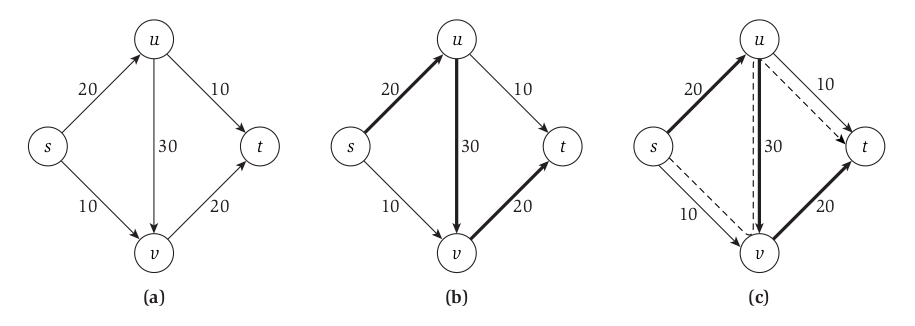
\includegraphics[width = 12 cm]{capitoli/network_flow/imgs/flow2.png}
  \caption{Nella figura (a) vediamo il grafo originale e nella (b) la soluzione trovata provando ad utilizzare un approccio greedy. Nella figura (c) vediamo invece quello che sarebbe la soluzione esatta per il problema del massimo flusso.}
\end{figure}

\subsection{The Residual Graph}
Dato una flow network $G$, e un flusso $f$ su $G$, definiamo il
\textbf{grafo residuale} $G_f$ di $G$ rispetto a $f$ come segue.
(Vedi grafo residuo (c) del flusso sulla Figura precedente dopo aver
spinto 20 unità di flusso lungo il percorso $s, u, v, t$.)

\begin{myblockquote}
  \begin{itemize}
    \item  L'insieme dei nodi di $G_f$ è uguale a quello di $G$.
    \item Per ogni arco $e = (u, v)$ di $G$ su cui
          $f(e) < c_e$ , ci sono $c_e - f(e)$ unità di capacità
          \emph{``rimanenti''} su cui potremmo provare a spingere il flusso in
          avanti. Quindi includiamo l'arco $e = (u, v)$ in $G_f$ , con una
          capacità di $c_e - f(e)$. Chiameremo gli archi inclusi in questo modo
          \textbf{forward edges}.
    \item Per ogni arco $e = (u, v)$ di $G$ su cui $f(e) > 0$, ci sono $f(e)$ unità di flusso che       possiamo ``\emph{annullare}'' se vogliamo, spingendo il flusso all'indietro (backward).         Quindi includiamo l'arco $e' = (v, u)$ in $G_f$ , con una capacità di $f(e)$. Notare che $e'$       ha le stesse estremità di $e$, ma la sua direzione è \textbf{invertita}; chiameremo gli archi       inclusi in questo modo \textbf{backward edges}.
  \end{itemize}
\end{myblockquote}

Si noti che ogni arco $e$ in $G$ può dare origine a uno o due archi
in $G_f$: Se $0 < f (e) < c_e$ risulta che sia un arco in avanti
che uno all'indietro siano inclusi in $G_f$ . Quindi $G_f$ ha al
massimo il doppio degli archi rispetto a $G$. A volte ci riferiremo
alla capacità di un arco nel grafo residuo come \textbf{residual
  capacity}, per aiutare a distinguerla dalla capacità dell'arco
corrispondente nella rete di flusso originale $G$.


\subsection{Augmenting Paths in a Residual Graph}

Ora vogliamo rendere preciso il modo in cui viene spinto il flusso da
$s$ a $t$ in $G_f$. Sia $P$ un cammino $s-t$ in $G_f$ (un
path nel grafo residuale viene chiamato \textbf{augmenting path}), cioè
$P$ non visita nessun nodo più di una volta. Definiamo
\texttt{bottleneck(P,\ f)} come la \textbf{minima capacità residua tra
  tutti gli archi di $P$}, rispetto al flusso $f$. Definiamo ora la
seguente operazione \texttt{augment(f\ ,\ P)}, che produce un nuovo
flusso $f'$ in $G$.

\begin{lstlisting}[language=Python, mathescape=true]
function augment(f, P) {
 Let b = bottleneck(P, f)

 For each edge (u, v) $\in$ P
    If e = (u, v) is a forward edge then
    	increase f (e) in G by b
  	Else ((u, v) is a backward edge, and let e = (v, u))
    	decrease f (e) in G by b
  	Endif
  Endfor

  Return(f)
}
\end{lstlisting}

Proprio per poter eseguire questa operazione abbiamo definito il grafo
residuale; per riflettere l'importanza dell'\textbf{augment} (aumento),
ci si riferisce a qualsiasi cammino $s-t$ nel grafo residuale come
\textbf{\emph{augmenting path}}. Il risultato di
\texttt{augment(f,\ P)} è un nuovo flusso $f'$ in $G$, ottenuto
aumentando e diminuendo i valori di flusso sugli archi di $P$.\\

Questa operazione di \textbf{augmentation} cattura il tipo di spinta
avanti e indietro (forward and backward) del flusso che abbiamo discusso
in precedenza. Consideriamo ora il seguente algoritmo per calcolare un
flusso $s-t$ in $G$.\\

\texttt{Max-Flow(G)}

\begin{lstlisting}[language=Python, mathescape=true]
function Max-Flow(G) {
	Start with f(e) = 0 for each edge e $\in$ E.

	While there is an s-t path in the residual graph $G_f$
  	  Find an s $\rightsquigarrow$ t path P in the residual network $G_f$
  	  $f'$ = augment(f , P)
  	  Update the residual graph $G_f$ using $f'$
	Endwhile

	Return f
}
\end{lstlisting}

Lo chiameremo Algoritmo di \textbf{Ford-Fulkerson}, dal nome dei due
ricercatori che lo svilupparono nel 1956.

\begin{figure}[H]
  \centering
  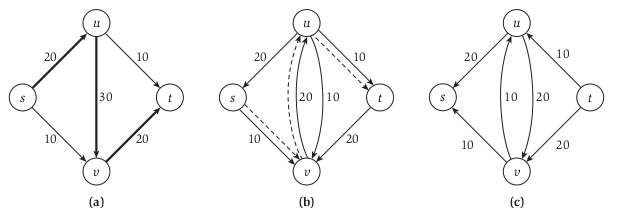
\includegraphics[width = 12 cm]{capitoli/network_flow/imgs/flow3.png}
  \caption{Esempio di un esecuzione dell'algoritmo di Ford Fulkerson}
\end{figure}

L'algoritmo Ford-Fulkerson è davvero molto semplice. Per quanto riguarda
il modo in cui vengono trovati i path nel grafo residuale, non è stato
specificato nell'algoritmo, ma si ha libera scelta sull'utilizzo di
algoritmi di esplorazione dei grafi, un esempio è l'utilizzo della DFS
(il costo complessivo dell'algoritmo di Ford-Fulkerson dipenderà anche
da questa scelta). Ciò che non è affatto chiaro è se il suo ciclo
\texttt{While} centrale termini e se il flusso restituito sia un flusso
massimo. Le risposte a entrambe queste domande si rivelano abbastanza
sottili.

\subsection{Analyzing the Algorithm: Termination and Running Time}

Per prima cosa consideriamo alcune proprietà che l'algoritmo mantiene
per induzione sul numero di iterazioni del ciclo \texttt{while},
basandoci sulla nostra ipotesi che tutte le \emph{capacità} siano numeri
interi.

\begin{myblockquote}
  Ad ogni stadio intermedio dell'algoritmo di Ford-Fulkerson, i valori di
  flusso $f(e)$ e le capacità residue in $G_f$ sono interi.
\end{myblockquote}

Possiamo usare questa proprietà per dimostrare che l'algoritmo di
Ford-Fulkerson termina. Per prima cosa mostriamo che il valore del
flusso aumenta strettamente quando applichiamo \emph{augmentation}.\\

\begin{minipage}{\textwidth}
  \begin{myblockquote}
    \begin{definition}\label{def:7.3}
      Sia $f$ un flusso in $G$, e sia $P$ un semplice cammino $s-t$ in
      $G_f$ . Allora $v(f') = v(f)$ + \texttt{bottleneck(P,\ f)}; e poiché
      \texttt{bottleneck(P,\ f)} \textgreater{} 0, abbiamo $v(f') > v(f)$.
    \end{definition}
  \end{myblockquote}
\end{minipage}

Abbiamo bisogno di un'altra osservazione per dimostrare la terminazione.
Dobbiamo essere in grado di limitare il massimo valore di flusso
possibile. Ecco un \textbf{upper bound}:

\begin{myblockquote}
  Se tutti gli archi al di
  fuori di $s$ potessero essere completamente saturati dal flusso, il
  valore del flusso sarebbe $\sum_{e \text{ out of }s} c_e$. Sia $C$
  questa somma. Quindi abbiamo $v(f) \le C$ per tutti i flussi $f$
  $s-t$
\end{myblockquote}

\paragraph*{Nota:} $C$ può essere un'enorme sovrastima del valore massimo
di un flusso in $G$, ma è utile per noi come limite finito.\\

Usando l'affermazione \ref{def:7.3}, ora possiamo dimostrare la terminazione:

\begin{myblockquote}
  Supponiamo, come sopra, che tutte le capacità nella rete
  di flusso $G$ siano numeri interi. Quindi l'algoritmo di
  Ford-Fulkerson termina al massimo in $C$ iterazioni del ciclo
  \texttt{while}.
\end{myblockquote}


\subsection{Costo}

Successivamente consideriamo il tempo di esecuzione dell'algoritmo
Ford-Fulkerson. Sia $n$ il numero di nodi in $G$, ed $m$ il numero
di archi in $G$. Abbiamo supposto che tutti i nodi abbiano almeno un
arco incidente, quindi $m \ge n/2$, e quindi possiamo usare
$O(m + n ) = O(m)$ per semplificare i limiti.

\begin{myblockquote}
  Supponiamo, come sopra, che tutte le capacità nella rete di flusso $G$
  siano numeri interi. Quindi l'algoritmo Ford-Fulkerson può essere
  implementato per funzionare in tempo $O(mC)$.
\end{myblockquote}

Una versione un po' più efficiente dell'algoritmo manterrebbe le linked
lists di archi nel grafo residuo $G_f$ come parte della procedura di
augmentation per il flusso $f$.


\section{Maximum Flows and Minimum Cuts in a Network}

Proseguiamo ora con l'analisi dell'algoritmo Ford-Fulkerson.


\subsection{Analyzing the Algorithm: Flows and Cuts}

Il nostro prossimo obiettivo è dimostrare che il flusso restituito
dall'algoritmo di Ford-Fulkerson ha il massimo valore possibile per il
flusso in $G$.\\

Per compiere progressi verso questo obiettivo, torniamo ad un problema
già descritto: \textbf{il modo in cui la struttura della rete di flusso
  pone upper bounds al valore massimo di un flusso $s-t$}. Abbiamo già
visto un upper bound:

\begin{myblockquote}
  il valore $v(f)$ di qualsiasi
  flusso $s-t$ $f$ è al massimo
  $C = \sum_{e \text{ out of } S} c_e$. A volte questo limite è utile,
  ma a volte è molto debole.
\end{myblockquote}

Usiamo ora la nozione di \textbf{taglio} per sviluppare un metodo molto
più generale per porre upper bound al valore del flusso massimo.

\begin{myblockquote}
  Si consideri la possibilità di dividere i nodi del grafo
  in due insiemi, $A$ e $B$, in modo che $s \in A$ e $t \in B$.

  Formalmente diciamo che un \textbf{taglio} $s-t$ è una
  partizione $(A, B)$ dell'insieme di vertici $V$, tale che
  $s \in A$ e $t \in B$.

  La \textbf{capacità di un taglio} $(A, B)$, che indicheremo con $c(A , B)$, è la somma delle
  capacità di tutti gli archi che escono da A:
  $
    c(A, B) = \sum_{e \text{ out of } A} c_e.
  $\\
  I tagli risultano fornire upper bounds molto naturali sui valori dei flussi.
\end{myblockquote}

Lo precisiamo attraverso una sequenza di teoremi e/o definizioni.

\begin{myblockquote}
  \begin{minipage}{\textwidth}
    \begin{definition}\label{def:7.6}
      Sia $f$ un flusso $s-t$ qualsiasi, e $(A, B)$ un taglio $s-t$, allora:
      $
        v(f) = f^{\text{out}}(A) - f^{\text{in}}(A)
      $
    \end{definition}
  \end{minipage}
\end{myblockquote}

Questa affermazione è in realtà molto più forte di un semplice upper
bound. Dice che osservando la quantità di flusso che $f$ invia
attraverso un taglio, possiamo misurare esattamente il valore del
flusso: \textbf{è la quantità totale che lascia A, meno la quantità che
  ``torna indietro'' in A}.\\

Se $A = {s}$, allora $f^{out}(A) = f^{out}(s)$ e $f^{in}(A) = 0$
poiché non ci sono archi che entrano nella sorgente per ipotesi. Quindi
l'affermazione per questo insieme $A = {s}$ è esattamente la
definizione del valore del flusso $v(f)$. Si noti che se $(A, B)$ è
un taglio, allora gli archi entranti in $B$ sono esattamente gli archi
che escono da $A$. Allo stesso modo, gli archi che escono da $B$
sono esattamente gli archi che entrano in $A$. Quindi abbiamo
$f^{out}(A) = f^{in}(B)$, semplicemente confrontando le definizioni di
queste due espressioni. Quindi possiamo riformulare la \ref{def:7.6} nel modo
seguente.

\begin{myblockquote}
  \begin{minipage}{\textwidth}
    \begin{definition}\label{def:7.7}
      Sia $f$ un flusso $s-t$ qualsiasi, e $(A, B)$ un taglio $s-t$, allora
      $
        v(f) = f^{\text{in}}(B) - f^{\text{out}}(B)
      $
    \end{definition}
  \end{minipage}
\end{myblockquote}

Se poniamo $A = V - {t}$ e $B = {t}$ nella \ref{def:7.7}, abbiamo
$v(f) = f^{in}(B) - f^{out}(B) = f^{in}(t) - f^{out}(t)$. In base alla
nostra assunzione il \textbf{sink} $t$ non ha archi uscenti, quindi
abbiamo $f^{out}(t) = 0$. Questo dice che avremmo potuto definire
originariamente il \emph{valore} di un flusso altrettanto bene in
termini del sink $t$: è $f^{in}(t)$, la quantità di flusso che
arriva al \textbf{sink}.\\

Una conseguenza molto utile della \ref{def:7.6} è il seguente upper bound.

\begin{myblockquote}
  \begin{minipage}{\textwidth}
    \begin{definition}\label{def:7.8}
      Sia $f$ un flusso $s-t$ qualsiasi, e $(A, B)$ un taglio $s-t$, allora
      $
        v(f) \le c(A, B)
      $
    \end{definition}
  \end{minipage}
\end{myblockquote}

In un certo senso, la \ref{def:7.8} sembra più debole della \ref{def:7.6},
poiché è solo una disuguaglianza piuttosto che un'uguaglianza. Tuttavia, ci sarà
estremamente utile, poiché il suo lato destro è indipendente da un flusso
particolare $f$. Quello che dice la \ref{def:7.8} è che \textbf{il valore di
  ogni flusso è limitato superiormente dalla capacità di ogni taglio}. In altre
parole, se eseguiamo un qualsiasi taglio $s-t$ in $G$ di un certo valore
$c^{*}$, sappiamo immediatamente dalla \ref{def:7.8} che non può esserci un
flusso $s-t$ in $G$ di valore maggiore di $c^{*}$. Al contrario, se valutiamo un
qualsiasi flusso $s-t$ in $G$ di un certo valore $v^{*}$, sappiamo
immediatamente dalla \ref{def:7.8} che non può esserci un taglio $s-t$ in $G$ di valore
minore di $v^{*}$.

\section{Analyzing the Algorithm: Max-Flow Equals Min-Cut}

Sia $\bar{f}$ il flusso restituito dall'algoritmo di
\textbf{Ford-Fulkerson}. Vogliamo dimostrare che $\bar{f}$ ha il
massimo valore possibile di qualsiasi flusso in $G$, e lo facciamo con
il metodo discusso sopra: Lo facciamo con un taglio $s-t$
$(A^{*} , B^{*})$ per il quale $v(\bar{f}) = c(A^{*} , B^{*})$. Questo
stabilisce immediatamente che $\bar{f}$ ha il valore massimo di
qualsiasi flusso, e che $(A^{*} , B^{*})$ ha la capacità minima di
qualsiasi taglio $s-t$.\\

L'algoritmo di Ford-Fulkerson \textbf{termina quando il flusso $f$ non
  ha un cammino $s-t$ nel grafo residuale $G_f$}. Questa risulta
essere l'unica proprietà necessaria per dimostrare la sua massimalità.

\begin{myblockquote}
  \begin{minipage}{\textwidth}
    \begin{definition}\label{def:7.9}
      Se $f$ è un flusso $s-t$ tale che non esiste un cammino $s-t$ nel
      grafo residuale $G_f$ , allora esiste un taglio $s-t$
      $(A^{*} , B^{*})$ in $G$ per cui $v(f) = c(A^{*} , B^{*})$. Di
      conseguenza, $f$ ha il valore massimo di qualsiasi flusso in $G$, e
      $(A^{*} , B^{*})$ ha la capacità minima di qualsiasi taglio $s-t$ in
      $G$.
    \end{definition}
  \end{minipage}
\end{myblockquote}


\begin{proof}
  Dobbiamo identificare un taglio che dimostri la precedente proprietà. A
  tal fine, indichiamo con $A^{*}$ l'insieme di tutti i nodi $v$ in
  $G$ per i quali esiste un cammino $s-v$ in $G_f$. Sia $B^{*}$
  l'insieme di tutti gli altri nodi: $B^{*} = V - A^{*}$.\\

  Per prima cosa stabiliamo che $(A^{*} , B^{*})$ è effettivamente un taglio
  $s-t$. È chiaramente una partizione di $V$. La sorgente $s$
  appartiene ad $A^{*}$ poiché c'è sempre un cammino da $s$ a $s$.
  Inoltre, $t \notin A^{*}$ assumendo che non ci sia un cammino $s-t$
  nel grafo residuale; quindi $t \in B^*$ come desiderato.\\

  Supponiamo ora che $e = (u, v)$ sia un arco in $G$ per il quale
  $u \in A^{*}$ e $v \in B^{*}$, come mostrato nella Figura seguente.
  Affermiamo che $f(e) = c_e$. Infatti, in caso contrario, $e$
  sarebbe un arco \emph{forward} nel grafo residuale $G_f$, e poiché
  $u \in A^{*}$ esiste un cammino $s-u$ in $G_f$; aggiungendo $e$ a
  questo cammino, otterremmo un cammino $s-v$ in $G_f$,
  contraddicendo la nostra ipotesi che $v \in B^{*}$.\\

  Supponiamo ora che $e' = (u' , v')$ sia un arco in $G$ per cui
  $u' \in B^{*}$ e $v' \in A^{*}$. Affermiamo che $f(e') = 0$. In caso
  contrario, $e'$ darebbe luogo a un arco \emph{backward}
  $e'' = (v' , u')$ nel grafo residuale $G_f$, e poiché
  $v' \in A^{*}$, allora è un cammino $s-v'$ in $G_f$; aggiungendo
  $e''$ a questo cammino, otterremmo un cammino $s-u'$ in $G_f$,
  contraddicendo la nostra ipotesi che $u' \in B^{*}$.\\

  Quindi tutti gli archi uscenti da $A^{*}$ sono completamente saturati di
  flusso, mentre tutti gli archi entranti in $A^{*}$ sono completamente
  inutilizzati. Possiamo ora usare la \ref{def:7.6} per raggiungere la conclusione
  desiderata:
  $$
    v(f) = f^{out}(A^{*}) - f^{in}(A^{*}) = \sum_{e \text{ out of }A^{*}} f(e) - \sum_{e \text{ into }A^{*}}f(e) = \sum_{e \text{ out of }A^{*}} c_e - 0 = c(A^{*}, B^{*})
  $$
\end{proof}

\begin{figure}[H]
  \centering
  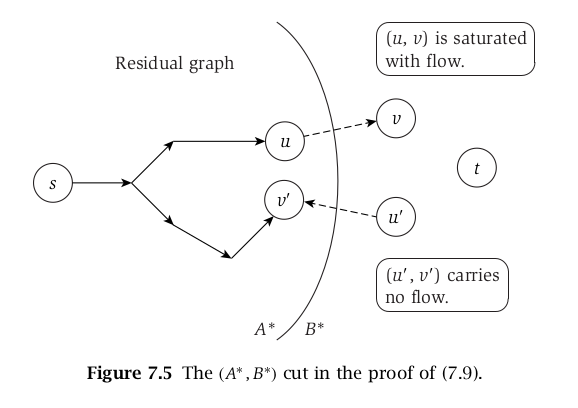
\includegraphics[width = 10 cm]{capitoli/network_flow/imgs/flow4.png}
  \caption{La dimostrazione della \ref{def:7.9}}
\end{figure}

\begin{myblockquote}
  \begin{minipage}{\textwidth}
    \begin{definition}\label{def:7.10}
      Il flusso $\bar{f}$ restituito dall'algoritmo di Ford-Fulkerson è un
      flusso massimo.
    \end{definition}
  \end{minipage}
\end{myblockquote}
\begin{myblockquote}
  \begin{minipage}{\textwidth}
    \begin{definition}\label{def:7.11}
      Dato un flusso f di valore massimo, possiamo calcolare un taglio $s-t$
      di capacità minima in tempo $O(m)$.
    \end{definition}
  \end{minipage}
\end{myblockquote}
\begin{myblockquote}
  \begin{minipage}{\textwidth}
    \begin{definition}\label{def:7.12}
      In ogni rete di flussi esiste un flusso $f$ e un taglio $(A, B)$
      tale che $v(f) = c(A, B)$.
    \end{definition}
  \end{minipage}
\end{myblockquote}

Il punto è che $f$ nella \ref{def:7.12} deve essere un flusso massimo $s-t$;
poiché se ci fosse un flusso $f'$ di valore maggiore, il valore di
$f$ supererebbe la capacità di $(A, B)$, e ciò contraddirebbe la
\ref{def:7.8}. Allo stesso modo segue che $(A, B)$ nella \ref{def:7.12} è un taglio
minimo (nessun altro taglio può avere capacità minore) perché se ci
fosse un taglio $(A , B)$ di capacità minore, sarebbe minore del
valore di $f$ , e anche questo contraddirebbe la \ref{def:7.8}. A causa di
queste implicazioni, la \ref{def:7.12} è spesso chiamata \textbf{teorema del
  taglio minimo del flusso massimo} ed è formulata come segue.

\begin{myblockquote}
  \begin{minipage}{\textwidth}
    \begin{theorem}[\textbf{Taglio Minimo e Flusso Massimo}]
      In ogni rete di flussi, il valore massimo di un flusso $s-t$ è
      uguale alla capacità minima possibile per un taglio $s-t$.
    \end{theorem}
  \end{minipage}
\end{myblockquote}